% !TeX spellcheck = en_US
\chapter{Implementation} % Main chapter title

\label{chap:implementation} % Change X to a consecutive number; for referencing this chapter elsewhere, use \ref{ChapterX}

\lhead{Chapter \ref*{chap:implementation}. \emph{Implementation}} % Change X to a consecutive number; this is for the header on each page - perhaps a shortened title

% \begin{lstlisting}[label={lst:swapoff}, caption={Bash commands for turning off swapping in Linux Debian}]
% \end{lstlisting}

\section{Containerization of Services}
Container images are provided for running the application inside the \ac{CRI}. Definition of the container manifest is done in the \enquote{Containerfile}\footnote{Containerfile: https://www.mankier.com/5/Containerfile} format.

\subsection{Code changes on core application}
For containerizing the \ac{OT} application, several changes were applied to its code base. This improves error handling and error tracing of the application and therefore simplifies development of the cluster. In the following sections, the several code changes are described in detail.

\subsubsection*{Introduction of exit codes}
The microservice \ac{DLL} files have return codes for different error cases. This is, for instance a code 200 in the \ac{AUTH} for connection issues to the database. As with process exit codes, a zero return code indicates a successful termination. Even though the main executable \enquote{open\_twin.exe} retrieves the return code, it did not convert these codes into proper process exit codes. 
Exit-Codes are a crucial part of the \ac{K8s}'s life cycle management as described in \autoref{chap:design.life_cycle}. Therefore, the return codes need to be converted into process exit codes.

\begin{lstlisting}[label=lst:code_changes.exitcodes.before, caption={Former code snippet from main executable for calling the microservice library code in Rust (\textit{/Microservices/OpenTwin/src/main.rs})}, language=rust, firstnumber=85]
let _result = initialize(siteid_c_str.as_ptr(), service_c_str.as_ptr(), db_c_str.as_ptr(), dir_c_str.as_ptr());
\end{lstlisting}
The surrounding lines of code in the main executable are shown in \autoref{lst:code_changes.exitcodes.before}\footnote{The code listings in this thesis have the corresponding file mentioned as part of the caption. Furthermore, their line numbers are aligned to the corresponding file.}. It calls the initialization method of the microservice \ac{DLL}, passes all its parameters and retrieves its return code.

\begin{lstlisting}[label=lst:code_changes.exitcodes.after, caption={Code changes in Rust main executable for additional treatment of exit codes (\textit{/Microservices/OpenTwin/src/main.rs})}, language=rust, firstnumber=86]
if _result != 0 {
  eprintln!("Library/Service initialization ({}:init()) failed with exit code {}", lib_path, _result);
  std::process::exit(_result);
}
\end{lstlisting}
A new condition for non-zero exit codes was added as shown in \autoref{lst:code_changes.exitcodes.after}. The variable \tcode{\_result}  contains the returned exit code of the library \ac{DLL}, whereas \tcode{lib\_path} contains the path to the library \ac{DLL}. As can be seen, it is used to describe the affected service name in a error message (line 87).
 
\subsubsection*{Debug verbosity in launcher}
By default Rust programs show a window for console output no matter if it was built in release mode or with debug parameters. However, the main executable uses conditional compilation to set configuration attributes about the windows subsystem.
\begin{lstlisting}[label=lst:cond_compilation_windows_subsystem, caption={Conditional compilation for disabling console output in non-debug builds (\textit{/Microservices/OpenTwin/src/main.rs})}, language=rust, firstnumber=2]
#![cfg_attr(not(debug_assertions), windows_subsystem = "windows")]
\end{lstlisting}
Rust provides a compilation option \tcode{debug\_assertions} that is set to \enquote{true} for compilations without code optimization\cite{Rust.20230209}. Therefore it is set to \enquote{true} if the application runs in debug mode. As shown in \autoref{lst:cond_compilation_windows_subsystem} with conditional compilation, this build option is checked and console output is only shown for debug builds. If the windows subsystem is set to \tcode{windows}, no console windows are rendered after starting the application.

Even if output is shown on the console window for debug builds only, the error messages are not able to be read conveniently in cases where the application crashes. This impedes debugging and diagnosis of regular application errors outside of a containerized environment.
To avoid this behavior, the launcher batch files were adapted. For this, a new parameter was invented to the batch file for running the batch file in verbose mode.
\begin{lstlisting}[label=lst:launcher_extension.parameter_validation.after, caption={Additional command argument for preventing close of window after termination (\textit{/Microservices/Launcher/OpenTwin\_session.bat})}, language=cmd, firstnumber=18]
IF "%~1"=="/V" (
  REM OT is opening console windows in debug build, so we want to pause them at the end
  SET pause_prefix=cmd.exe /S /C "
  SET pause_suffix=" ^& pause
  ECHO ON
)
\end{lstlisting}
As first step, a new command line argument has been introduced. If \enquote{/V} is appended to the start of the launcher batch file it will run with higher verbosity.  As can be seen in \autoref{lst:launcher_extension.parameter_validation.after}, with \enquote{/V} appended, two new variables \tcode{pause\_prefix} and \tcode{pause\_suffix} are set (line 20-21). Furthermore, command output is enabled to debug the launcher file itself (line 22).

\begin{lstlisting}[label=lst:launcher_extension.call.after, caption={Additional command extension for preventing close of window after termination (\textit{/Microservices/Launcher/OpenTwin\_session.bat})}, language=cmd, firstnumber=34]
START "AUTHORIZATION SERVICE" %pause_prefix%open_twin.exe AuthorisationService.dll <*@ \Suppressnumber @*>
  "%OPEN_TWIN_SERVICES_ADDRESS%:%OPEN_TWIN_AUTH_PORT%" "%OPEN_TWIN_MONGODB_ADDRESS%"
  "%OPEN_TWIN_MONGODB_PWD%"%pause_suffix% <*@ \Reactivatenumber @*>
\end{lstlisting}
The newly defined variables \tcode{pause\_prefix} and \tcode{pause\_suffix} are then appended to the command of starting a service. This is shown in \autoref{lst:launcher_extension.call.after}. It ensures that a service process is started in a new window and the command is followed by the \ac{Windows} \enquote{pause} command to stop and wait for user interaction. Thus, the user is now able to read error messages if application crashes occur.

\subsubsection*{Enhanced logging and error tracing}
For improving the error tracing, the overall log amount has been increased. This involves enabling the logging of the central logging functions inside the library \enquote{OpenTwinCommunication}. The logging mechanism did not use logging to standard output. Instead, calls to the respective functions for logs were just ignored. This was changed and logging to standard output has been introduced. 
\begin{lstlisting}[label=lst:implementation.log_message_filter, caption={Comparison of the set log level with the log severity of the message. If the converted log severity is less than the defined log level, the message is ignored. (\textit{/Libraries/OpenTwinCommunication/src/ServiceLogger.cpp})}, language=c++, firstnumber=60]
if (((int)_severity) < ((int)m_logLevel)) {
	return;
}
\end{lstlisting}
Log messages also have information stored about their severity that can be converted from \enquote{enum} values to their numeric representation. With respect of the high amount of printed log messages, they are now filtered by their severity. This filter mechanism is shown in \autoref{lst:implementation.log_message_filter}.

Additionally, more calls to the logging mechanism, including caller information, have been added. For instance, the \ac{AUTH} now shows error messages for caught exceptions and errors during database initialization.
Also, the general error tracing has been improved. In the main services \ac{GSS}, \ac{LSS} and \ac{AUTH}, exception handling has been added, where it was not present before. Furthermore, the formatting of exception messages was improved and more information has been added.

For the current time being, there is an ongoing work to replace the logging to standard output by forwarding the log lines to a central logging library.

\subsubsection*{Certificate changes}
Since \ac{OT} is using \ac{mTLS} for communication between services, the \ac{CSR} file needs to contain the host specification for the outgoing \ac{IP} address and host name. Thus, in \ac{OT} a batch script substitutes placeholders in a template \ac{CSR} file. The respective section of the \ac{CSR} template is shown in \autoref{lst:implementation.mtls_csr_replacement}.
\begin{lstlisting}[label=lst:implementation.mtls_csr_replacement, caption={Variables defined in the \ac{CSR} are substituted by their respective values. (\textit{/Deployment/\hspace{0.01em}Certificates/server-csr\_template.json})}, language={}, firstnumber=3]
  "hosts": ["$HOSTNAME$", "$IP_ADDRESS$", "localhost", "127.0.0.1"],
\end{lstlisting}
However, this process does not work if performed for a containerized application. If the replacement takes place during the creation of the container, the final host name or \ac{IP} address does not yet exist. If, on the other hand, the automatic replacement is done later, it cannot be carried out from outside the container, as the script automatically replaces only the local host name.
To solve this problem, the \ac{CSR} template was extended by fixed values for \enquote{localhost} and \enquote{127.0.0.1}. This already covers the majority of use cases. Additionally, it is recommended to not generate the certificate as part of the container image build process. Instead it should be inserted via a file mount.

\subsubsection*{Listening on all interfaces}
Container images have a certain network image for communicating to external hosts. Processes inside the container have to bind to this network interface. However, the \ac{IP} address of this network interface is unpredictable during compile time. The processes that run inside a container therefore have to bind to all available network interfaces to be accessible to the outer network which is performed by binding on the address \enquote{0.0.0.0}.
Moreover, the services exchange service information with other services as described in \autoref{chap:background.baseline_architecture}. Because the binding address \enquote{0.0.0.0} is invalid and not accessible from the public, it must differ from this published address in a containerized environment.

Instead of binding to all network interfaces, the main executable in \ac{OT} was only able to bind to a given \ac{IP} address (based on the published service address) only. Also, it was not possible to configure a different binding address than the one published to other services.

\begin{lstlisting}[label=lst:listen_all_interfaces.before, caption={Listener binding before the applied changes (\textit{Microservices/OpenTwin/src/main.rs})}, language=rust, firstnumber=145, numbers=left]
let listener = net::TcpListener::bind(&service_url).await?;
println!("Starting server at {:?}", service_url);
\end{lstlisting}
\autoref{lst:listen_all_interfaces.before} shows the affected lines of code in the main executable. The passed argument for the service \ac{URL} is forwarded to the server listener class. Afterwards, the address is printed on the console. The service \ac{URL}, here passed as variable, consists of the service address and the port of the service.

To not affect the outer interface, the changes work with the data already provided. This means, the passed arguments to the main executable are not altered.
\vspace{4em}
\begin{lstlisting}[label=lst:listen_all_interfaces.after, caption={Listener binding after the applied changes. The service url is parsed, based on its port. Binding is done on all interfaces. (\textit{Microservices/OpenTwin/src/main.rs})}, language=rust, firstnumber=150]
let service_port = Url::parse(&format!("https://{}", service_url))
.expect(&format!("Invalid service url. Unable to parse service url: {}", service_url))
.port();
if service_port.is_none() {
	panic!("Invalid service url. Service url is lacking port defintion: {}", service_url);
}
let binding_address = format!("0.0.0.0:{}", service_port.unwrap().to_string());
let listener = net::TcpListener::bind(&binding_address).await?;
println!("Server listening on {:?} (publishing {:?})", binding_address, service_url);
\end{lstlisting}
The binding address is separated from the published address, since the address in the argument still gets passed to the microservice \ac{DLL}. Afterwards, the service \ac{URL} is processed as shown in \autoref{lst:listen_all_interfaces.after}. First, the given service \ac{URL} is parsed and the port number is extracted (lines 150-152). If no port is found or the parsing failed, the application fails and shows an error (lines 153-155). Afterwards, the port number is concatenated with the binding address \enquote{0.0.0.0} and therefore the server binds to all addresses (lines 156-157). The last line shows the new output containing the port number and the address published to other services.


\subsection{Container definition}
There were three container images prepared for containerization of \ac{OT}. These cover the main services for \ac{GSS}, \ac{LSS} and \ac{AUTH}. The structure is the same for each of the container files. The first part of the container file is shown in \autoref{lst:containerfile.1}.
\begin{lstlisting}[label=lst:containerfile.1, caption={Containerfile for the \ac{LSS}. Description of the base image and variable tagging using a build argument. (\textit{Distribution/Container/session.Containerfile})}, language=docker, firstnumber=1]
ARG BASE_IMAGE_TAG=ltsc2022
FROM mcr.microsoft.com/windows/servercore:$BASE_IMAGE_TAG
\end{lstlisting}
The first line introduces a build argument for defining the target image tag from the command line without altering the container file.  It is used afterwards to pass the image tag to the base container image. The subsequent lines define labels for the resulting image.
\vspace{1em}
\begin{lstlisting}[label=lst:containerfile.3, caption={Containerfile for the \ac{GSS}. Description of the command line and certificate creation. (\textit{Distribution/Container/session.Containerfile})}, language=docker, firstnumber=21]
ENTRYPOINT ["cmd", "/C"]
CMD ["open_twin.exe", "SessionService.dll", "0", \
"%OPEN_TWIN_LSS_SERVICE_ADDRESS%:%OPEN_TWIN_LSS_PORT%", \
"%OPEN_TWIN_GSS_SERVICE_ADDRESS%:%OPEN_TWIN_GSS_PORT%", \
"%OPEN_TWIN_AUTH_PORT%"]
EXPOSE 8093
WORKDIR C:/app/Deployment/Certificates
COPY ./ ../
RUN createCertificate.bat && certutil -addstore root %OPEN_TWIN_CA_CERT%
WORKDIR C:/app/Deployment
RUN C:\app\Deployment\VC_Redist\VC_redist.x64.exe /install /quiet && \<*@ \Suppressnumber @*>
    move opengl32sw.dll opengl32.dll<*@ \Reactivatenumber @*>
\end{lstlisting}
\autoref{lst:containerfile.3} shows the lower section of the container file for containerizing the \ac{LSS}.
The container files differ in the runtime specification. They run the same entry point, but have a different process running as command. Besides, the exposed port depends on the service inside the container. 
After defining the command and copying the files into the container image (lines 22-28), the certificates are built as part of the image file system (line 29).
Since the compute services are dependent to C++ libraries that are not present in the base image, the Microsoft Visual C++ Redistributable must be installed as well (line 31).
The second command of this line performs the renaming of the OpenGL software rendering \ac{DLL}. This is necessary, because OpenGL version 2.0 is not available inside the container.

% Container image must be built on each node machine manually. Since the Windows base image os is only compatible with the respective host \ac{OS}.
% Deployment-Verzeichnis muss dafür initial auf Node kopiert werden.
% -TODO: (Skript ("setup-node") dafür schreiben, was neusten release von github zieht (RUN download?) und image autom. baut + image pusht?)  - base image (FROM) mittels args dynamisch gestalten?


\section{Cluster Setup}
The following section describes the setup of different nodes in the cluster. While the master node refers to the \ac{K8s} control plane node which is responsible for distribution of the workers, the worker nodes are the actual machines that are executing the applications.
The used version of \ac{K8s} is \enquote{v1.25.3}. The version of ContainerD is \enquote{v1.6.8}, on both sides, the worker nodes and the master node.

\subsection{Setting up the master node}
For setting up the master node on Linux, a system based on Debian Bullseye 11.5 was used. Basis for the performed steps is the \ac{K8s} documentation for setting up a container runtime\cite{Kubernetes.2019} and the online tutorial of Basappa\cite{Basappa.2022}.

\subsubsection{Installing prerequisites and ContainerD}
After installing and setting up the \ac{OS}, the swap mechanism needs to be permanently turned off. This is done by editing the file system table (\tcode{fstab}), in file \tcode{/etc/fstab} respectively, by commenting out the swap partitions and masking the systemd swap units as shown in \autoref{lst:disable_swap}.
\begin{lstlisting}[label=lst:disable_swap, caption={Bash commands for disabling Swap mechanism and masking.}, language=bash]
$ sed -i '/ swap / s/^\(.*\)$/#\1/g' /etc/fstab
$ systemctl mask dev-sda3.swap
\end{lstlisting}

The container runtime requires certain kernel features to be enabled. On Debian 11, the required kernel modules for virtual networking facilities (\tcode{br\_netfilter}) and overlay filesystems (\tcode{overlay}) are not enabled by default. Thus, they have to be manually enabled.
% To permanently enable them and keep them enabled after reboot, the setting is stored in a file as shown in \autoref{lst:kernel_modules}.
To permanently enable them and keep them enabled across reboots, the setting is stored in a file in the directory for loaded modules (\textit{/etc/modules-load.d/k8s.conf}).
\begin{comment}
% https://www.natarajmb.com/2022/06/kubernetes-debian/
\begin{lstlisting}[label=lst:kernel_modules, caption={Bash commands for enabling required kernel modules.}, language=bash]
$ cat <<EOF | sudo tee /etc/modules-load.d/k8s.conf 
overlay 
br_netfilter 
EOF 
\end{lstlisting}
\end{comment}

For functional networking on the master node, \ac{K8s} also requires internal network packets being forwarded to the pods. Additionally, the tracking table for tracing network packets and their assigned connection is increased. This is a prerequisite for the applied \ac{NAT} which is used in container networking.
New files with respective settings are created in the directory for kernel settings as shown in \autoref{lst:ip_forward}.
\begin{lstlisting}[label=lst:ip_forward, caption={Bash commands for enabling \ac{IP} forwarding and network filtering.}, language=bash]
$ cat <<EOF | tee /etc/sysctl.d/k8s.conf 
  net.bridge.bridge-nf-call-iptables  = 1
  net.bridge.bridge-nf-call-ip6tables = 1
  net.ipv4.ip_forward                 = 1 
  net.netfilter.nf_conntrack_max      = 524288 
EOF
$ echo 1 > /proc/sys/net/ipv4/ip_forward
\end{lstlisting}

After installing ContainerD with all its prerequisites from the package registry, a configuration file (\tcode{config.toml}) is created.
Subsequently, the SystemD \ac{cgroup} is added to the runtime options of ContainerD and its service is restarted. For this, the commands from \autoref{lst:master.containerd_config} are applied.
\vspace{1em}
\begin{lstlisting}[label=lst:master.containerd_config, caption={Bash command for setting up containerd config},language=bash, morekeywords={sudo, kubeadm, tee, service}]
$ containerd config default | <*@ \Suppressnumber @*>
  sed 's/\[plugins.\"io.containerd.grpc.v1.cri\".containerd.runtimes.runc.options\]/&\n SystemdCgroup = true/' | tee /etc/containerd/config.toml >/dev/null <*@ \Reactivatenumber @*>
$ service containerd restart
\end{lstlisting}

To finally start the cluster, the packages for the Kubelet service, \enquote{kubeadm} and \enquote{kubectl} need to be installed. Then, the cluster can be initialized by running the command line tool as shown in \autoref{lst:master.kubeadm.init}. Since the configuration parameters can also be passed as YAML file, this is the preferred method of passing arguments and allows version control of the required configuration.
\begin{lstlisting}[label=lst:master.kubeadm.init, caption={Bash command for setting up the cluster}, morekeywords={sudo, kubeadm}, numbers=none]
$ kubeadm init --config kubeadm_config.yaml
\end{lstlisting}

Since Flannel is used as network overlay, the \ac{IP} address range provided for pods must be \enquote{10.244.0.0/16}\cite{GitHubKubernetesSIGWindowsTools.20230213}. Additionally, a value is provided that sets the \ac{CRI} socket address for newly registered nodes to the one of ContainerD. Furthermore, the \ac{cgroup} driver for the Kubelet service on worker nodes is set to SystemD. Thus, the \ac{cgroup} driver on Linux worker nodes should be aligned to the master node.
The information passed as configuration is presented in \autoref{lst:master.kubeadm.config}.
\begin{lstlisting}[label=lst:master.kubeadm.config, caption={YAML configuration for providing configuration for the cluster and newly registered ndoes. (\textit{Distribution/Controlplane/kubeadm\_config.yaml})}, language=yaml]
kind: ClusterConfiguration
apiVersion: kubeadm.k8s.io/v1beta3
kubernetesVersion: v1.25.3
networking:
  podSubnet: "10.244.0.0/16" # pod-network-cidr
---
kind: InitConfiguration
apiVersion: kubeadm.k8s.io/v1beta3
nodeRegistration:
  criSocket: unix:///var/run/containerd/containerd.sock
---
kind: KubeletConfiguration
apiVersion: kubelet.config.k8s.io/v1beta1
cgroupDriver: systemd
\end{lstlisting}


\subsubsection{Applying a Container Network Interface}
After successfully initializing the cluster, the overlay network for Flannel must be set up.
For this, the respective entity description can be directly downloaded from the vendor\footnote{Flannel entity description: \href{https://raw.githubusercontent.com/flannel-io/flannel/master/Documentation/kube-flannel.yml}{https://raw.githubusercontent.com/flannel-io/flannel/master/Documentation/kube-flannel.yml}}. Since networking has to blend with Flannel on \ac{Windows}, the \ac{VNI} (4096) and port (4789) for Flannel on \ac{Windows} must be set as part of the configuration. For this, manual editing of the description must be performed. The respective values are added to the configuration map section where the network configuration file is described (the section \enquote{net-conf.json} of \enquote{kube-flannel.yml}) as shown in \autoref{lst:implementation.flannel_fixup}. This file is automatically created on newly registered nodes. The changed entity description is applied on the cluster respectively.
\begin{lstlisting}[label=lst:implementation.flannel_fixup, caption={Fixup for Flannel manifest. Here the values \tcode{VNI} and \tcode{Port} were added. (\textit{kube-flannel.yml})}]
net-conf.json: | {
  "Network": "10.244.0.0/16",
  "Backend": {
    "Type": "vxlan",
    "VNI" : 4096,
    "Port": 4789
}}
\end{lstlisting}
\vspace{-2em}
\subsubsection{Adding the proxy daemon sets}\vspace{-1em}
The usage of \ac{Windows} worker nodes in a \ac{K8s} cluster requires additional configuration mappings and daemon sets to be applied on the cluster. Those are used for setting up a proxy for Flannel. The \ac{SIG} \enquote{Windows Tools} of \ac{K8s} provides the additional objects\cite{GitHubKubernetesSIGWindowsTools.20230213}. Before applying them, a replacement of the \ac{K8s} version and the Flannel version is performed. This procedure is achieved by running the two commands shown in \autoref{lst:master.proxy_daemonsets}. 
\begin{lstlisting}[label=lst:master.proxy_daemonsets, caption={Bash command for adding the flannel overlay configuration\cite{GitHubKubernetesSIGWindowsTools.20230213}}, language=bash]
$ curl -L https://raw.githubusercontent.com/kubernetes-sigs/sig-windows-tools/master \<*@ \Suppressnumber @*>
  /hostprocess/flannel/kube-proxy/kube-proxy.yml | 
  sed 's/KUBE_PROXY_VERSION/v1.25.3/g' | 
  kubectl apply -f -<*@ \Reactivatenumber @*>
$ curl -L https://raw.githubusercontent.com/kubernetes-sigs/sig-windows-tools/master \<*@ \Suppressnumber @*>
  /hostprocess/flannel/flanneld/flannel-overlay.yml | 
  sed 's/FLANNEL_VERSION/v0.17.0/g' | 
  kubectl apply -f -<*@ \Reactivatenumber @*>
\end{lstlisting}


\subsection{Setting up the worker node}\label{chap:implementation.setup_worker}
The initialization of the worker node is mainly oriented on the guide for adding \ac{Windows} nodes that is provided from the \ac{SIG} \enquote{Windows Tools} on GitHub\cite{GitHubKubernetesSIGWindowsTools.20230213}. Although there is an original guide from \ac{K8s}\cite{Kubernetes.20220419}, it was not used as basis because it is outdated.

First, the node preparation scripts of the \ac{K8s} \ac{SIG} \enquote{Windows Tools} are retrieved and executed as shown in \autoref{lst:worker.sig_scripts}. The first script retrieved (\textit{Install-Containerd.ps1}) installs ContainerD and its prerequisites on \ac{Windows}. Installation of the prerequisites involves the Windows features \enquote{Hyper-V}, \enquote{Hyper-V Tools}, \enquote{Hyper-V for PowerShell} and \enquote{Containers}. Once the features are installed and the system has successfully rebooted, the script has to be restarted. It then proceeds by downloading the binary of ContainerD and adding its location to the \tcode{PATH} environment variable. ContainerD's configuration file is changed to align the \ac{CNI} file locations with \ac{K8s}. The script ends by registering ContainerD as a service.

The second script (\textit{PrepareNode.ps1}) prepares the node for joining the cluster. It first downloads the Kubelet executable and creates a script file that is called by the Kubelet service. The created script file contains runs the Kubelet in consideration of version dependent command arguments. Afterwards, the \ac{NSSM}\footnote{NSSM: https://nssm.cc/} is downloaded and the Kubelet script is registered as a service. Finally, the \textit{PrepareNode} script also sets up firewall rules for Kubelet.

Furthermore the command line tools \enquote{kubectl}, \enquote{kubeadm}, \enquote{crictl} and \enquote{nerdctl} are installed. While installing \enquote{crictl}, it is added to the \tcode{PATH} environment variable.

\begin{lstlisting}[label=lst:worker.sig_scripts, caption={Retrieval of node preparation scripts\cite{GitHubKubernetesSIGWindowsTools.20230213}}, language=PowerShell, morekeywords={curl.exe, Install-Containerd.ps1, PrepareNode.ps1}]
> curl.exe -LO https://raw.githubusercontent.com/kubernetes-sigs/sig-windows-tools/master/kubeadm/scripts/Install-Containerd.ps1
> .\<*@\textbf{Install-Containerd.ps1}@*>
> curl.exe -LO https://raw.githubusercontent.com/kubernetes-sigs/sig-windows-tools/master/kubeadm/scripts/Prepare<*@\kern.7pt@*>Node.ps1
> .\PrepareNode.ps1 -KubernetesVersion v1.25.3
\end{lstlisting}

% \begin{comment}
%service.
%% [plugins."io.containerd.grpc.v1.cri"].sandbox_image
%For having a valid image at a later point in time, the \ac{CRI} value \tcode{sandbox\_image} in ContainerD's configuration file (\textit{config.toml}) needs to be replaced with a newer version.
%
%After successfully setting up the \ac{NAT} and installing ContainerD as a service, the node will be finally prepared to host tasks. For this, another Powershell script \enquote{PrepareNode}\footnote{https://github.com/kubernetes-sigs/sig-windows-tools/releases/download/v0.1.5/PrepareNode.ps1} from the Kubernetes \ac{SIG} runs. After running the script, the resulting \enquote{StartKubelet} file needs to be changed to drop invalid arguments.
%
%% C:\k\kubelet.exe $global:KubeletArgs --cert-dir=$env:SYSTEMDRIVE\var\lib\kubelet\pki --config=/var/lib/kubelet/config.yaml --bootstrap-kubeconfig=/etc/kubernetes/bootstrap-kubelet.conf --kubeconfig=/etc/kubernetes/kubelet.conf --hostname-override=$(hostname)
%Furthermore, the following lines were added to the Kubelet configuration:
%\begin{lstlisting}[label=lst:master.configtoml_changes, caption={Configuration changes in ContainerD configuration file (\textit{config.toml})\cite{GitHubKubernetesSIGWindowsTools.20230213}}]
%enforceNodeAllocatable: []
%cgroupsPerQOS: false
%enableDebuggingHandlers: true
%\end{lstlisting}
%These configuration values are valid for \ac{Windows} machines only and cause an error in Kubelet on Linux. The configuration changes therefore can only be served to Windows machines and the configuration on the nodes needs to be changed locally.
%\end{comment}


% Es wurde "New-HnsNetwork -Type NAT -Name nat -Gateway 10.244.0.1 -AdressPrefix 10.244.240.0/20" ausgeführt
% TODO: Evtl. testen, ob man mit Docker auf Netzwerk zugreifen kann? "Object already exists"
% TODO: -- siehe: https://github.com/kubernetes-sigs/sig-windows-tools/issues/128

After successfully running the preparation script the node should be ready to join the cluster. For joining the cluster a token is generated on the master node. The token is copied to the preapared node and used as part of a \enquote{join} command. \autoref{lst:worker.join} shows the command for joining the cluster, whereas the token is substituted by \enquote{TOKEN}.
\begin{lstlisting}[label=lst:worker.join, caption={Command for joining new nodes on Windows}, language=PowerShell, morekeywords={kubeadm.exe}]
> kubeadm.exe join 1.2.3.4:6443 --token TOKEN --discovery-token-ca-cert-hash sha256:HASH \<*@ \Suppressnumber @*>
  --cri-socket "npipe:////./pipe/containerd-containerd"<*@ \Reactivatenumber @*>
\end{lstlisting}
Besides containing the token and the master node's \ac{IP} address, the command also has the hash value of the \ac{CA} of the master node. For \ac{K8s} versions \enquote{v1.25} and below the command also requires the explicit declaration of ContainerD as container runtime. Thus, the additional option \tcode{cri-socket} is defined.

The successful join of the node is verified by running \tcode{kubectl get nodes} on the master node. This prints the newly added node.


\section{Automatic setup}
% TODO: Powershell script beschreiben
Even though the scripts provided from the \ac{SIG} \enquote{Windows Tools} cover most of the preparation steps, some manual steps are still required as described in the respective guide\cite{GitHubKubernetesSIGWindowsTools.20230213}. To automate the preparation process where possible, and to also provide tools for debugging error cases, further steps are required. Thus, a custom script (\textit{Distribution/Container/setup-node.ps1}) was created to provide this aid.

The script automates the process of rebooting and rerunning the preparation after the required \ac{Windows} features are installed, and provides instructions for steps that cannot be automated. It also checks the prerequisites before performing any action. This means, it is checked whether the \ac{OS} is \enquote{\ac{Windows} Server} and if a certain minimum version of \ac{Windows} is used. The check for prerequisites is shown in \autoref{lst:auto.check_preq}.
\begin{lstlisting}[label=lst:auto.check_preq, caption={Powershell commands in the automated setup script. Checks for prerequisites.}, language=PowerShell]
	if (-not ((Get-ComputerInfo).WindowsProductName | Select-String "Server")) {
		throw "Prerequisites not met. Windows Server is required as operating system."
	}
	if (-not (Get-Hotfix -ErrorAction Ignore KB4489899)) {
		if (-not ([System.Environment]::OSVersion.Version -gt [System.Version]"10.0.17763.0")) {
			throw "Prerequisites not met. You either need KB4489899 installed, or a Windows Version higher than 10.0.17763"
		}
	}
\end{lstlisting}

Besides checking for system requirements, the custom script also installs tools for debugging. This includes the \ac{Windows} version of \enquote{kubeadm} and \enquote{kubectl}, as well as the command line tools for debugging containers on \ac{Windows}, namely \enquote{crictl} and \enquote{nerdctl}.
Furthermore, the custom script also excludes the ContainerD process from the \ac{Windows} Defender firewall as shown in \autoref{lst:auto.win_defender}. This increases the pull and general runtime performance of containers.
The installation of the command line tools also involves setting up PowerShell auto completion and include to the \tcode{PATH} environment variable.
\begin{lstlisting}[label=lst:auto.win_defender, caption={Powershell command in the automated setup script. Exclusion of all actions performed by containerd.exe from Windows Defender.}, language=PowerShell, numbers=none]
	Add-MpPreference -ExclusionProcess "$Env:ProgramFiles\containerd\containerd.exe"
\end{lstlisting}


\subsection{Cluster design}
Adding worker nodes to the existing cluster was probed in three different scenarios. Starting point of the investigation was the most complex approach (\autoref{fig:implementation.cluster-scenario.1}). The complexity of the system was subsequently reduced in order to break down errors that were related to networking, the encrypted communication and the host-process isolation.
Those scenarios are described here more in detail.

The first scenario, as seen in \autoref{fig:implementation.cluster-scenario.1}, is the most complex one. The two physical computers shown in the figure represent the machines where the \ac{K8s} nodes are running. Here, \enquote{Physical computer 1 (PC1)} is a local Linux machine in the role of the control plane, whereas \enquote{Physical computer 2 (PC2)} is a high-performance computer for running the worker. Because PC2 is located in the university and therefore access restricted, the organizationally simplest approach was to set up a \ac{VM} on PC2. The \ac{VM} then had unrestricted access. The \ac{K8s} compute node is set up in this \ac{VM}.
Both physical machines are connected to the Internet and not within the same network. Instead of accessing PC2 directly via a public \ac{IP} address, both computers have to be connected to a \ac{VPN}. \ac{VPN} is a technology, where network traffic is encrypted to enable access to an internal network from the outside.

\begin{figure}[ht]
	\centering
	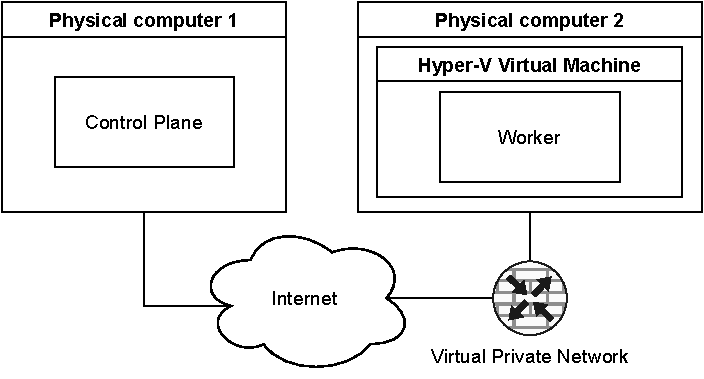
\includegraphics[width=.8\textwidth]{Figures/Cluster-scenarios-1.pdf}
	\caption{Cluster design scenario where worker node is running on a dedicated machine inside the protected University network. Additionally, the worker node is hosted inside a \ac{VM} to have another isolation layer and full admin privileges on the worker node.}
	\label{fig:implementation.cluster-scenario.1}
\end{figure}

The problems in the first scenario is the additional abstraction layer between Hyper-V \ac{VM} for administer the worker node and the physical machine. This involves additional network interfaces that translate the addresses from within the \ac{VM} to the external network. Misconfiguration in one of those layers can hinder the start of host-process containers that try to bind on these network interfaces.

The second scenario is shown in \autoref{fig:implementation.cluster-scenario.2}. Here, the worker is not inside a \ac{VM} and runs bare metal. The physical computers are still only accessible within the \ac{VPN} and not located in the same network.
\begin{figure}[ht]
\centering
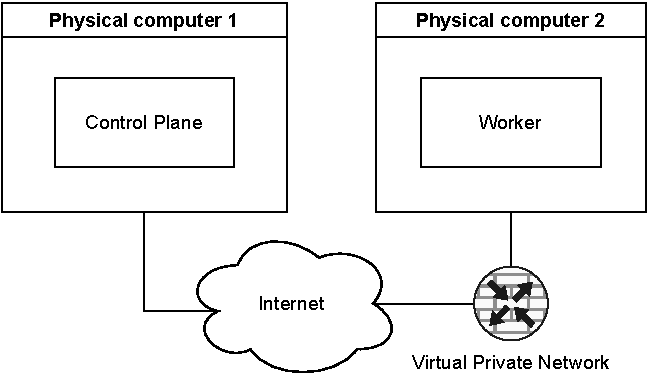
\includegraphics[width=.8\textwidth]{Figures/Cluster-scenarios-2.pdf}
\caption{Cluster design scenario where worker node is running on a dedicated machine inside the protected University network.}
\label{fig:implementation.cluster-scenario.2}
\end{figure}
Since the \ac{VPN} is still necessary for the connection between PC1 and PC2, this caused problems in the connection between Control Plane and worker node. While implementing the second scenario, \ac{IP} addresses could not be assigned by \ac{K8s}. After starting the containers, the \ac{HCS} threw the error \enquote{IP address is either invalid or not part of any configured subnet(s)}. This was justified by the \ac{VPN} network interface, since it has to support a large amount of subnets.

This leads to the third scenario, shown in \autoref{fig:implementation.cluster-scenario.3}, which is the simplest. Here, the two physical computers are connected directly in the same network. Since this expects mostly the real world scenario this is the preferable one. In this scenario, the containers were able to start and got an \ac{IP} address assigned.
\begin{figure}[hb]
	\centering
	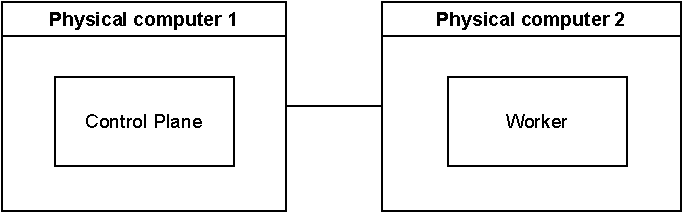
\includegraphics[width=.8\textwidth]{Figures/Cluster-scenarios-3.pdf}
	\caption{Cluster design scenario where master and worker node were both running on a dedicated physical machine each.}
	\label{fig:implementation.cluster-scenario.3}
\end{figure}


\subsection{Deployment of the application}
As a first draft, only the \ac{LSS} of the application is deployed. 
Deployment of the application is done by applying the manifest as shown in \autoref{lst:deploy.yaml}.
The manifest defines a pod using the container image of the \ac{LSS} (lines 2-4). Since the images are not yet provided via an image registry, the images are stored locally. Thus, the \ac{K8s} is directed to never pull the image and retrieve it locally instead.
The passed environment variables (lines 5-13) are defined by the section \tcode{env}, whereas the variable \tcode{OPEN\_TWIN\_LSS\_SERVICE\_ADDRESS} is set with the \ac{IP} address of the pod. The external port is defined as 8093, which is equivalent to the port of the \ac{LSS}.
The node selector property (lines 16-17) defines a requirement for the node scheduler to select only \ac{Windows} nodes.
The manifest is applied on the cluster using \tcode{kubectl apply}.
\begin{lstlisting}[label=lst:deploy.yaml, caption={Partial section of configuration for cluster deployment of the \ac{LSS} (\textit{Distribution/Kubernetes/open\_twin.yaml})}, language=yaml]
containers:
- name: opentwin-session
  image: local.dev/opentwin-session:latest
  imagePullPolicy: Never
  env:
    - name: OPEN_TWIN_LSS_SERVICE_ADDRESS
      valueFrom:
        fieldRef:
          fieldPath: status.podIP
    - name: OPEN_TWIN_MONGODB_ADDRESS
      value: 1.2.3.4:27017
    - name: OPEN_TWIN_GSS_SERVICE_ADDRESS
      value: 5.6.7.8
  ports:
  - containerPort: 8093
nodeSelector:
  kubernetes.io/os: windows
\end{lstlisting}

